\documentclass{standalone}

\usepackage[english]{babel}

% to use colors

\usepackage{xcolor}

% to define font size

\usepackage{amsfonts}
\usepackage{ulem}
\usepackage{moresize}
\usepackage{anyfontsize}

% to use tikz and its libraries

\usepackage{tikz-timing}
\usepackage{tikz}

\usetikzlibrary{backgrounds}
\usetikzlibrary{decorations.pathreplacing, positioning, calc, arrows, shapes, automata, petri, patterns}

% to use tikzmark, to place and refer to marks outside the current figure

\tikzset{every picture/.style={remember picture}}

% styles for transitions

\tikzset{transition/.append style={fill=black!20, thick}}
\tikzset{transition/.append style={fill=black!20, thick}}

% styles for test and inhib arcs.

\tikzstyle{test}=[pre, *-]
\tikzstyle{inhib}=[pre, o-]

%%%%%%%%%%%%%%%%%%%%%%%%%%%%%%%%%%%%%%%%%%%%%%%%%%
%                  BEGIN DOCUMENT                %
%%%%%%%%%%%%%%%%%%%%%%%%%%%%%%%%%%%%%%%%%%%%%%%%%%

\begin{document}

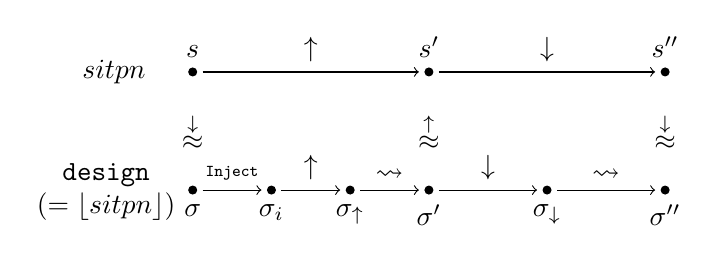
\begin{tikzpicture}

  % SITPN STATE NODES

  \node (sitpn) {$sitpn$};
  \node[draw, circle, inner sep=1pt, fill=black, label={above:$s$}] (s) at ($(sitpn)+(1,0)$){};
  \node[draw, circle, inner sep=1pt, fill=black, label={above:$s'$}] (sprime) at ($(s)+(3,0)$) {};
  \node[draw, circle, inner sep=1pt, fill=black, label={above:$s''$}] (ssnd) at ($(sprime)+(3,0)$) {};

  \draw ($(s.east)+(2pt,0)$) edge[->] node [midway, above] {$\uparrow$} ($(sprime.west)-(2pt,0)$);
  \draw ($(sprime.east)+(2pt,0)$) edge[->] node [midway, above] {$\downarrow$} ($(ssnd.west)-(2pt,0)$);

  % VHDL DESIGN NODES

  \node (vhdld) at ($(sitpn)-(.1,1.5)$) {
    \begin{tabular}{@{}c@{}}
      $\mathtt{design}$ \\
      ($=\lfloor{}sitpn\rfloor$)\\
    \end{tabular}
  };

  \node[draw, circle, inner sep=1pt, fill=black, label={below: $\sigma$}] (sig) at ($(s)-(0,1.5)$) {};
  \node[draw, circle, inner sep=1pt, fill=black, label={below: $\sigma'$}] (sigprime) at ($(sprime)-(0,1.5)$) {};
  \node[draw, circle, inner sep=1pt, fill=black, label={below: $\sigma_i$}] (sigi) at ($(sig)+(1,0)$) {};
  \node[draw, circle, inner sep=1pt, fill=black, label={below: $\sigma_\uparrow$}] (sigup) at ($(sigprime)-(1,0)$) {};
  
  \node[draw, circle, inner sep=1pt, fill=black, label={below: $\sigma''$}] (sigsnd) at ($(ssnd)-(0,1.5)$) {};
  % \node[draw, circle, inner sep=1pt, fill=black, label={below: $\sigma'_i$}] (sigprimei) at ($(sigprime)+(1,0)$) {};
  \node[draw, circle, inner sep=1pt, fill=black, label={below:
    $\sigma_\downarrow$}] (sigdw) at ($(sigsnd)!.5!(sigprime)$) {};

  \draw ($(sig.east)+(2pt,0)$) edge[->] node [midway, above] {\ssmall$\mathtt{Inject}$} ($(sigi.west)-(2pt,0)$);
  \draw ($(sigi.east)+(2pt,0)$) edge[->] node [midway, above] {$\uparrow$} ($(sigup.west)-(2pt,0)$);
  \draw ($(sigup.east)+(2pt,0)$) edge[->] node [midway, above] {$\rightsquigarrow$} ($(sigprime.west)-(2pt,0)$);
  
  \draw ($(sigprime.east)+(2pt,0)$) edge[->] node [midway, above] {$\downarrow$} ($(sigdw.west)-(2pt,0)$);
  % \draw ($(sigprimei.east)+(2pt,0)$) edge[->] node [midway, above] {$\downarrow$} ($(sigdw.west)-(2pt,0)$);
  \draw ($(sigdw.east)+(2pt,0)$) edge[->] node [midway, above] {$\rightsquigarrow$} ($(sigsnd.west)-(2pt,0)$);  

  % STATE SIMILARITY RELATION
  
  \node at ($(s.south)!.5!(sig.north)$) {$\stackrel{\downarrow}{\approx}$};
  \node at ($(sprime.south)!.5!(sigprime.north)$) {$\stackrel{\uparrow}{\approx}$};
  \node at ($(ssnd.south)!.5!(sigsnd.north)$) {$\stackrel{\downarrow}{\approx}$};
  
\end{tikzpicture}

\end{document}